\scanpage{58}
\mspage{28}
\deleted{\unsure{(72)|(71)}} et. l'action de $\Gamma_{\underline G}=\Gamma$ sur $\widehat M_G\simeq\widehat M_{g_{\alpha_0},\widehat I_{\alpha_0}}$ est triviale si $g_{\alpha_0}=1$, et elle se fait à travers
\diagram{\begin{tikzcd}[ampersand replacement=\&]
\text{(72)}\quad\Gamma_{\underline G}\arrow[r]\&\mathfrak S_{\widehat I_{\alpha_0}}\quad(\simeq\mathfrak S_4)
\end{tikzcd}}
dans le cas où $g_{\alpha_0}=0$. L'image de $\Gamma_{\underline G}$ dans $\mathfrak S_4$ doit pouvoir être n'importe quel sous-groupe de $\mathfrak S_4$, sauf erreur. Explicitons déjà quels sont les cas où la dim. ambiante est $\leq2$. Le cas de la dim ambiante $1$ \inserted{i.e. où la codim modulaire \inserted{$s_1$} de $\underline G$ est $0$,} est évidemment celui donné par (70), où $G$ est réduit à un sommet isolé.

Considérons donc le cas de la dim mod ambiante $2$, i.e. codim modulaire $1$, i.e. \uline{une} arête. On trouve soit
\figure{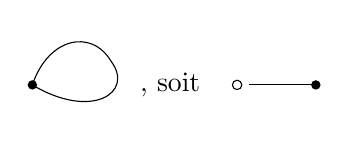
\begin{tikzpicture}[baseline=-.1cm]
\draw (0,0) .. controls (.2,.6) and (.75,.72) .. (1.0,.3) .. controls (1.3,-.1) and (.75,-.45) .. (0,0);
\fill (0,0) circle(1.7pt);\node at (1.75,0) {, soit};
\draw (2.75,0)--(3.6,0);\draw (2.6,0) circle(1.7pt);\fill (3.6,0) circle(1.7pt);
\end{tikzpicture}}.
\inserted{On trouve les trois cas de dim modulaire} \deleted{Dans le cas $g_{\alpha_0}=0$ tous les sommets sauf $1$ sont d'ordre $\unsure{<|2}$} ambiante $2$, dim modulaire $1$
\margin{MD-graphes de dim mod $1$, dim. modulaire ambiante $2$.}
\figure{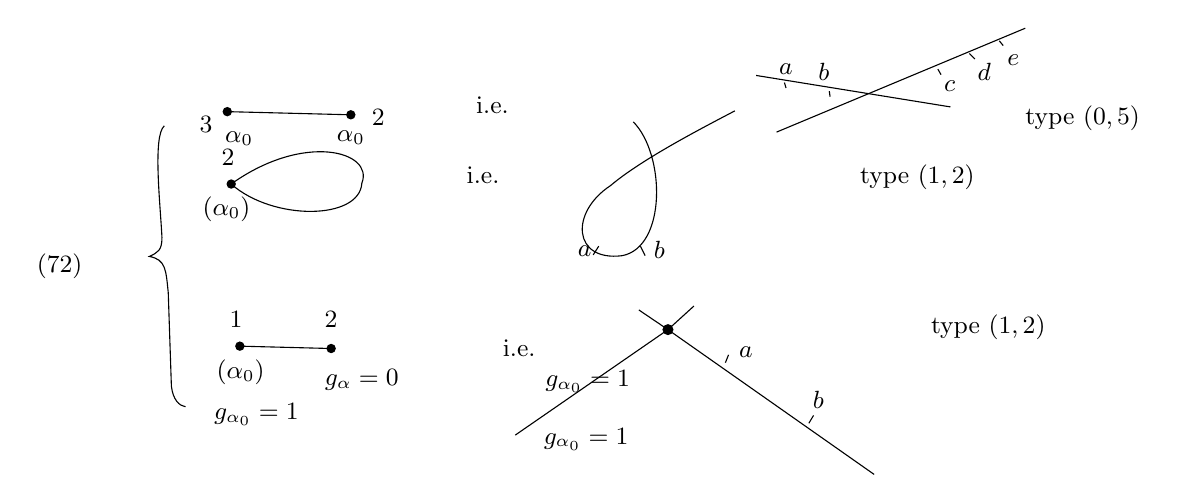
\begin{tikzpicture}[x=.010cm,y=-.010cm,every node/.style={font=\small}]
\node at (-150,310) {$(72)$};
\draw (-17,132) .. controls (-32,145) and (-22,232) .. (-20,274) .. controls (-20,290) and (-25,293) .. (-36,298) .. controls (-15,302) and (-15,315) .. (-12,344) -- (-8,463) .. controls (-6,480) and (2,488) .. (10,489);
% First graph and its curve.
\draw (63,114)--(220,118);\fill (63,114) circle(1.7pt);\fill (220,118) circle(1.7pt);
\node at (36,130) {$3$};\node at (78,148) {$\alpha_0$};\node at (255,122) {$2$};\node at (220,147) {$\deleted{\unsure{\alpha_0}}$};\node at (400,106) {i.e.};
\draw (735,68)--(982,108);\draw (761,140)--(1077,8);
\draw (771,77)--(773,84);\node at (773,60) {$a$};
\draw (828,88)--(829,95);\node at (821,64) {$b$};
\draw (966,60)--(970,67);\node at (981,82) {$c$};
\draw (1006,40)--(1013,47);\node at (1025,63) {$d$};
\draw (1044,24)--(1049,30);\node at (1062,48) {$e$};\node at (1150,123) {type $(0,5)$};
% Second graph and its curve.
\draw (68,206) .. controls (160,140) and (250,164) .. (234,205) .. controls (231,252) and (121,253) .. (68,206);\fill (68,206) circle(1.7pt);
\node at (64,172) {$2$};\node at (62,238) {$(\alpha_0)$};\node at (388,195) {i.e.};
\draw (579,127) .. controls (620,169) and (621,286) .. (565,297) .. controls (502,305) and (498,242) .. (550,208) .. controls (590,174) and (670,133) .. (708,113);
\draw (535,285)--(528,296);\node at (517,291) {$a$};\draw (588,285)--(594,297);\node at (612,290) {$b$};\node at (940,198) {type $(1,2)$};
% Third graph and its curve.
\draw (79,412)--(195,415);\fill (79,412) circle(1.7pt);\fill (195,415) circle(1.7pt);
\node at (74,378) {$\deleted{\unsure{1}}$};\node at (195,378) {$2$};\node at (80,445) {$(\alpha_0)$};\node at (100,499) {$g_{\alpha_0}=1$};\node at (234,455) {$g_\alpha=0$};\node at (434,414) {i.e.};
\draw (429,525)--(623,391)--(656,361);\draw (586,366)--(623,391)--(885,575);\fill (623,391) circle(2pt);
\node at (521,457) {$\deleted{\unsure{g_{\alpha_0}}=1}$};\node at (519,530) {$g_{\alpha_0}=1$};
\draw (696,433)--(700,423);\node at (722,420) {$a$};\draw (802,510)--(808,500);\node at (814,480) {$b$};\node at (1030,388) {type $(1,2)$};
\end{tikzpicture}}
(NB les sommets, ou branches des courbes, dont le genre \inserted{ou poids marqué} n'est pas marqué en dessous, sont de genre \inserted{ou poids marqué} zéro; les poids marqués sont indiqués sur le graphe \unsure{au|en} dessus des sommets)
\margin{57}
